\NextFile{UsingExtensions.html}
\chapter{Using MATSim Extensions}

\subsubsection{Introduction}

The default MATSim releases contain all the functionality typically  used to model agent behavior and simulate traffic. But sometimes, this  just is not enough. The MATSim Extensions provide additional  functionality for specific tasks, and can be used along MATSim. \href{http://www.matsim.org/extensions}{MATSim Extensions}  gives an overview of the currently available extensions. Please note  that these extensions are usually provided and maintained by single  persons from the community, and thus long-term support may vary from the  default MATSim release.

\subsubsection{Downloading Extensions}

All extensions come as a compressed zip-file. You can either download  the last stable release of an extension to be used together with the  stable release of MATSim, or you can download a so-called "nightly  build"—an automatically created, but untested and probably unstable  version of the extension.
\begin{itemize}
	\item You can download the stable releases of extensions from \href{http://sourceforge.net/projects/matsim/files/MATSim/}{SourceForge}.
	\item Likely unstable nightly builds can be downloaded from our \href{http://matsim.org/files/builds/}{nightly builds directory}.
	\item Make sure to also download MATSim itself. The extensions cannot be used without MATSim.
\end{itemize}

\subsubsection{Using Extensions on the Command Line}

Once you've downloaded an extension and MATSim, unzip the extension  and place the extension's directory inside the MATSim directory, next to  the 
\texttt{libs} directory. The file/directory structure should look similar to the following example:
\begin{verbatim}
matsim/
+ MATSim.jar
+ libs/
| + $<$lots of .jar files$>$
+ extension1/
| + extension1.jar
+extension2/
| + extension2.jar
| + libs/       $<$-- not all extensions contain additional libs
| | + $<$one or more .jar files$>$
\end{verbatim}

Then, start your simulation with the extension.jar-file on the classpath along the MATSim jar-file, e.g:
\begin{verbatim}
java -Xmx512m -cp MATSim.jar:extension1/extension1.jar:extension2/extension2.jar org.matsim.run.Controler myConfig.xml


\end{verbatim}

On Windows, use 
\texttt{;} instead of 
\texttt{:} to separate the different jar-files.

\subsubsection{Using Extensions in Eclipse}

Unzip the downloaded extension and place the extension's directory in  your eclipse project. Then, add the extension's jar-file to the 
\texttt{Java Build Path} in Eclipse's 
\texttt{Project Settings}.

\subsubsection{Documentation about Specific Extensions}

Extensions are developed and documented by their maintainers. Not all extensions are listed below; see the \href{http://www.matsim.org/extensions}{list of available} extensions for their description and documentation.



\vfill\eject
\NextFile{GTFS2TransitSchedule.html}
\section{GTFS2TransitSchedule}

This guide whill show you how to convert GTFS data to a MATSim Transit Schedule

\subsubsection{Automatic conversion}
\begin{itemize}
	\item Put the set of GTFS files of each public transport system in a different folder of your file system.
	\item Create a java program that constructs an object of the class
\texttt{GGTFS2MATSimTransitSchedule}in the package 
\texttt{GTFS2PTSchedule} which is part of this extension.For this you need to specify:
\end{itemize}
\begin{enumerate}
	\item An array of folders (
\texttt{File} class) where your public transport system specifications are located.
	\item An array of Strings representing the network modes correspondent to each public transport defined in b) (e. g. “
\texttt{car}” for buses, “
\texttt{rail}” for metro).
	\item The MATSim network object with the nodes in latitude and longitude coordinates (
\texttt{WGS84}).
	\item An array of Strings with the names of the calendar services that are desired (e. g. “
\texttt{weekday}”, “
\texttt{daily}”). Remember that MATSim only simulates one day, but the GTFS files specify routes for many calendar days or dates.
	\item The desired output coordinates system
\end{enumerate}
\begin{itemize}
	\item Call the method 
\texttt{TransitSchedule getTransitSchedule()}.  Then, each route of each given public transit systems will be processed  with the semi-automatic procedure presented in the following figure.
\end{itemize}
\begin{figure}[htp]
	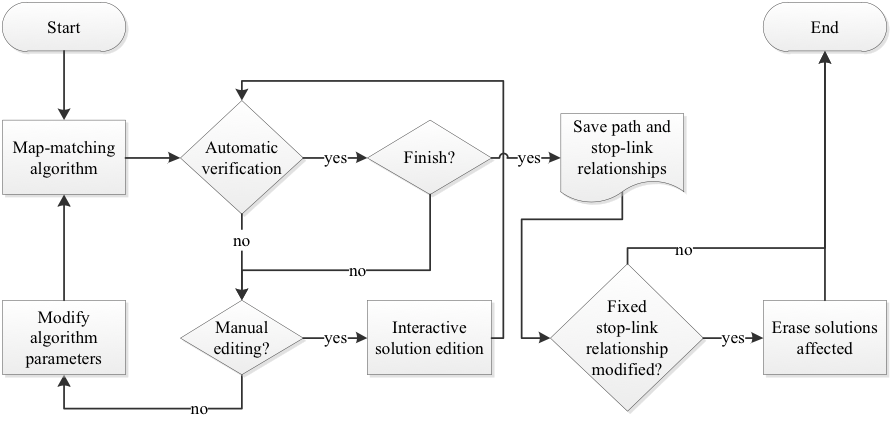
\includegraphics{figures/gtfs2schedule/gtfsAutoConversion.png}
\end{figure}




\subsubsection{Manual correction of automatic conversion}

For the manual editing process one can visualize, edit and verify the solution for each route:
\begin{itemize}
	\item Visualization: A navigation network is displayed, including all  relevant information for working with one single route. This includes  the route’s profile, the given sequence of GPS points and its current  solution (path and stop-link relationships). Selected elements are drawn  in a different color. All is displayed in a bi-dimensional interactive  way with refresh of the cursor location in the working coordinates, and  panning,  zoom and view-all options.
	\item Selection: Different options for selecting elements of the solution  or elements from the network are provided. It is possible to select the  nearest link (solution or network), nearest node (network) or nearest  stop (solution) to a point indicated by the user. When a stop that has a  stop-link relationship already, the corresponding link is selected as  well. If a link of the solution path is selected and it does not have a  subsequent link connected, a new one from the network is selected with  one click; the selected link is the one with the most similar angle than  the line defined by the end node of the initial link and a point  indicated by the user.
	\item Solution modification: The first link of the sequence can be added  selecting any link of the network. If a link of the solution path does  not have a subsequent link connected, it is possible to add one  according to the selection function described in (b). If there are two  subsequent links in the solution that are not connected (a gap), a  subsequence that connects the mentioned links is added, using the  shortest path algorithm, with the current parameters. Furthermore,  selecting one link of the path, it is possible to delete it, or to  delete all the links before or after it. Finally, stop-link  relationships can be modified selecting both elements. If the modified  relationship was fixed, the user  is prevented because the tool erase  the solutions of the routes to which the selected stop belongs.
	\item Network modification: New nodes to the road network can be added. In  addition, with any node selected, it is possible to add a new link  selecting the end node.
\end{itemize}

Hints and interaction details:
\begin{itemize}
	\item It is necessary to pass the verification process (“Is OK”) for saving a route result
	\item The routes are saved in temporal files located in the ./data/paths/ folder relative to the program location.
	\item Panning and zoom functions are provided dragging the mouse and moving the mouse wheel.
	\item View all function is provided typing the “v” key
	\item Up and down keys allow to select the next or previous link of the path.
	\item “$<$” or ”$>$” keys allow to select the previous or next stop 

\begin{figure}[htp]

\end{figure}
	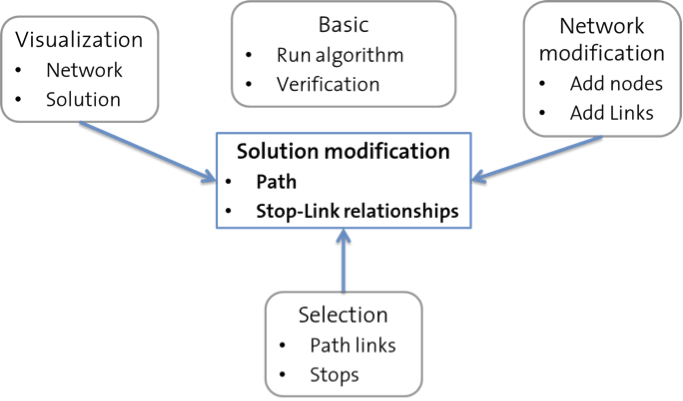
\includegraphics{figures/gtfs2schedule/gtfsManualEdit.png}
\end{itemize}

\subsubsection{Saving the converted data}

Finally, after the semi-automatic process, the Transit Schedule  object is returned and the network object is modified (splitting, new  nodes and links, and modes of the links). One can save in a XML  the 
\texttt{TransitSchedule} object constructing a 
\texttt{TransitScheduleWriter} object, and the modified network with a 
\texttt{NetworkWriter}.


\vfill\eject
\NextFile{MATSim4UrbanSim.html}
\section{MATSim4UrbanSim}

\subsection{Guide on UrbanSim usage of the travel model plug-in}

The current travel model plug-in implementation is applicable for the  Brussels zone, Zurich parcel, PSRC (Puget Sound Region Council) parcel  and Seattle parcel UrbanSim application.

Note that some of the instructions may change since the travel model plug-in is still under development.

\subsubsection{1 Prerequisites}

You must have installed UrbanSim, before getting started with the  travel model plug-in. The following provides an entry point to install  UrbanSim and continues with installation instructions for additional  software packages required by the travel model plug-in.

\subparagraph{Hints for installing UrbanSim}

To install UrbanSim please follow the UrbanSim Downloads and Installation Instructions on \href{http://urbansim.org/Download/}{http://urbansim.org/Download/}.

When installing OPUS and UrbanSim manually you can get the  installation instructions in "Downloading Sample Data and Source Code"  on: \href{http://urbansim.org/Download/DownloadingSampleDataAndSourceCode}{http://urbansim.org/Download/DownloadingSampleDataAndSourceCode}.

Windows users using the installer are getting the source code and data automatically.

Finally make sure that all UrbanSim environment variables, meaning  OPUS\_HOME, OPUS\_DATA\_PATH and PYTHONPATH, are set as described in the  installation instructions, see \href{http://urbansim.org/Download/SixtyFourBitMachines}{http://urbansim.org/Download/SixtyFourBitMachines} for Windows, \href{http://urbansim.org/Download/MacintoshInstallation}{http://urbansim.org/Download/MacintoshInstallation} for Mac or \href{http://urbansim.org/Download/LinuxInstallation}{http://urbansim.org/Download/LinuxInstallation} for Linux.

Note:  For using the travel model plug-in it is sufficient only to install the  required Python packages, i. e. numpy, scipy, lxml, sqlalchemy and  elixir.

\subparagraph{MATSim4UrbanSim prerequisites}

In addition to the UrbanSim installation the MATSim travel model plug-in requires the following software installed:
\begin{itemize}
	\item Java JDK 1.6 or newer: Download and install the newest version  of the Java SE Development Kit (JDK) for your operating system from \href{http://www.oracle.com/technetwork/java/javase/downloads/index.html}{http://www.oracle.com/technetwork/java/javase/downloads/index.html}. Make sure adding Java's /bin directory to the PATH environment variable. Click\href{http://java.com/en/download/testjava.jsp}{here}to test ifjavaisalready installed on your computer.
	\item Python XML Schema Bindings (PyXB): Download the PyXB 1.1.3 distribution file from \href{http://sourceforge.net/projects/pyxb/files/pyxb/1.1.3/}{http://sourceforge.net/projects/pyxb/files/pyxb/1.1.3/}  and extract it to a convenient place. Open a command prompt (Windows)  or a terminal (Mac, Linux). To install PyXB (this may requires  administrator or root privileges) go into the extracted directory and  type
\\


\texttt{python setup.py install}
\end{itemize}

\subsubsection{2 MATSim4UrbanSim installation}

This section describes how to install MATSim4UrbanSim.

\subparagraph{Automatic installation}

Make sure to have the Python lib directory included to the  PYTHONPATH. The Python lib directory is the directory that contains the  site-package directory that is already included in the PYTHONPATH. The  lib directory should be something like


\texttt{C:$\backslash$Python2.6$\backslash$Lib$\backslash$ }for Windows,


\texttt{/Library/Frameworks/Python.framework/Versions/2.6/lib/} for Mac or


\texttt{/usr/lib/python2.6/} for Linux (Ubuntu).

To install MATSim4UrbanSim open command prompt (Windows) or a  terminal (Mac, Linux) and navigate to opus\_matsim/configs in the opus  source directory. Than type


\texttt{python install\_matsim4urbansim.py}

This creates the subdirectories matsim4opus/jar, loads required  MATSim executables and libraries and configures them. After the  installation the file/directory structure should look something like  Figure 1.

To test whether the MATSim4UrbanSim installation was successful follow the instructions described in Section 2.3.

Note: The installer will replace jar-files and libraries from a previous MATSim4UrbanSim installation.

\subparagraph{Manual installation}

In case that the automatic installation does not work follow these instructions:
\begin{itemize}
	\item Create the following directory structure in OPUS\_HOME: OPUS\_HOME/matsim4opus/jar
	\item Download the following files from \href{http://www.matsim.org/files/builds/}{http://www.matsim.org/files/builds/} into the jar directory:   
\begin{itemize}
	\item MATSim\_rXXXXX.jar (where XXXXX refers the current revision)
	\item MATSim\_libs.zip
	\item matsim4urbansim-X.X.X-SNAPSHOT-rXXXXX.zip (where XXXXX refers the current revision)
\end{itemize}
	\item Rename MATSim\_rXXXXX.jar into "matsim.jar".
	\item Extract the zip files MATSim\_libs.zip and matsim4urbansim-X.X.X-SNAPSHOT-rXXXXX.zip. After that the zip files can be removed.
	\item Rename the directory matsim4urbansim-X.X.X-SNAPSHOT-rXXXXX into  "contrib". Than navigate into contrib and rename the jar-file  matsim4urbansim-X.X.X-SNAPSHOT.jar into "matsim4urbansim.jar".
\end{itemize}

Be careful when renaming files or directories (i. e. make sure  that everything is written in lower case and check for spelling errors).  After the installation the file/directory structure in the matsim4opus  directory should look something like Figure 1. To test whether the  MATSim4UrbanSim installation was successful follow the instructions  described in Section 2.3.

\subparagraph{Test your MATSim4UrbanSim installation}

To test your installation open a command prompt (Windows) or a  terminal (Mac, Linux) and navigate to opus\_matsim/tests in the opus  source directory (PYTHONPATH). Then type


\texttt{python travel\_model\_test.py}

This starts a test scenario. If the test completes without errors, your travel model plug-in should be working.

\begin{figure}[htp]
\includegraphics[width=\textwidth]{figures/matsim4urbansim/structure.png}
\caption{After the installation the matsim4opus directory should contain the depicted files and subdirectories.}
\end{figure}

\subsubsection{3 Using MATSim for UrbanSim}

This section aims to explain the MATSim travel model plug-in at the example of the Seattle\_parcel scenario.\textbf{}

\subparagraph{MATSim Data Requirements}

MATSim related input-files are:
\begin{itemize}
	\item a road network in MATSim format (mandatory)
	\item a plans file (optional)
\end{itemize}

These files are not included in the UrbanSim base\_year\_data and  must be added manually. To store these files create the red marked  folder structure as shown in Figure 2. This means store network files in  the "matsim/network" folder and the plans-files in the "matsim/plans"  folder.

For the current Seattle parcel example scenario you can download the zipped matsim folder \href{https://svn.vsp.tu-berlin.de/repos/public-svn/matsim/examples/countries/us/seattle/matsim.zip}{here.}  Unzip it into your OPUS\_DATA/seattle\_parcel/base\_year\_data/2000/  directory. After that your seattle\_parcel base\_year\_data should look  like Figure 2.

\begin{figure}[htp]
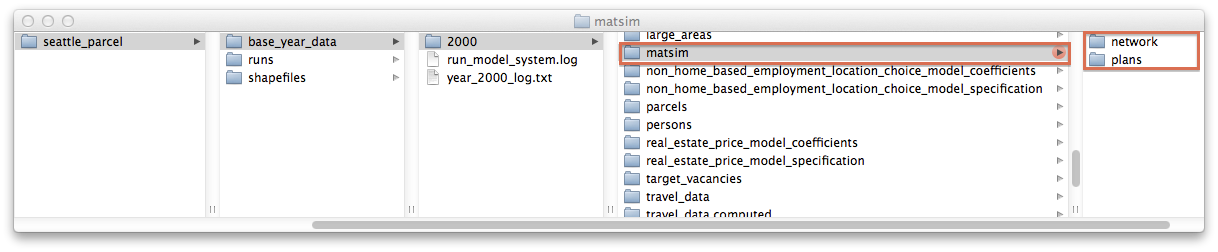
\includegraphics[width=\textwidth]{figures/matsim4urbansim/seattle_parcel_base_year_dir_v2.png}
\caption{Store MATSim related files like road networks and  plans-files directly in the base\_year\_data folder of the corresponding  UrbanSim application.}
\end{figure}

\subparagraph{UrbanSim Data Requirements}

In order to create input data for MATSim UrbanSim requires certain  data sets and attributes to reflect where a person lives and works.

\textbf{For UrbanSim parcel} applications the following data sets and attributes (in parenthesis) are required:
\begin{itemize}
	\item persons (person\_id, household\_id, job\_id)
	\item households (household\_id, building\_id)
	\item jobs (job\_id, building\_id)
	\item buildings (building\_id, parcel\_id)
	\item parcels (parcel\_id, x\_coord\_sp, y\_coord\_sp, zone\_id)
	\item zones (zone\_id)
\end{itemize}

\textbf{For UrbanSim zone} applications the following data sets and attributes (in parenthesis) are required:
\begin{itemize}
	\item persons (person\_id, household\_id, job\_id)
	\item households (household\_id, zone\_id)
	\item jobs (job\_id, zone\_id)
	\item zones (zone\_id, xcoord, ycoord)
\end{itemize}

\subparagraph{Travel Model Configuration Options}

In a recent effort a set of MATSim configuration parameters are  embedded into the travel\_parameter\_configuration section of the UrbanSim  configuration. This allows to configure MATSim in the OPUS GUI under  the Models tab as shown in Figure 3. The travel model conguration  section consists of a few lines of XML code and can be added into  existing UrbanSim configurations. A sample configuration for Seattle  parcel including the travel model configuration section can be  downloaded \href{https://svn.vsp.tu-berlin.de/repos/public-svn/matsim/examples/countries/us/seattle/seattle_parcel.xml}{here}.

\begin{figure}[htp]
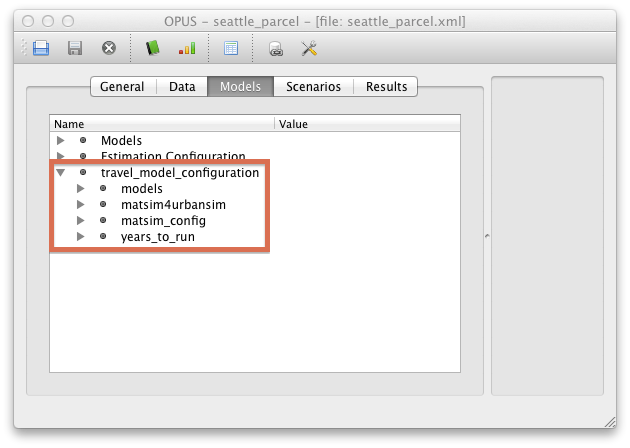
\includegraphics[width=\textwidth]{figures/matsim4urbansim/gui.png}
\caption{MATSim4UrbanSim configuration in OPUS GUI}
\end{figure}

The following explains step by step the MATSim configuration options provided by the OPUS GUI.

Launch the OPUS GUI and open the Seattle\_parcel sample configuration  (download see above). Switch to the Models tab to get to the travel  model configuration section as shown in Figure 4. The following  subsections are available:

\textbf{Models}:

The models section contains five models that couple MATSim with UrbanSim:
\begin{enumerate}
	\item \textbf{get\_cache\_data\_into\_matsim\_parcel} generates the MATSim input for UrbanSim parcel applications
	\item \textbf{get\_cache\_data\_into\_matsim\_zone} generates the MATSim input for UrbanSim zone applications
	\item \textbf{run\_travel\_model\_parcel }executes MATSim for UrbanSim parcel applications.
	\item \textbf{run\_travel\_model\_zone} executes MATSim for UrbanSim zone applications.
	\item \textbf{get\_matsim\_data\_into\_cache} imports the results of the traffic simulation for the next UrbanSim iteration (no distinction between parcel and zone here).
\end{enumerate}

To run MATSim for parcel applications enable the models \textbf{1},\textbf{ 3} and \textbf{5}. For UrbanSim zone applications use the models \textbf{2, 4} and \textbf{5}.

\textbf{MATSim4UrbanSim}:
\begin{itemize}
	\item \textbf{population\_sampling\_rate}: The population  sampling rate determines the percentage of considered travellers for a  MATSim run. For instance 0.01 means that only 1\% of travellers are  considered for the traffic simulation. This option allows to speed up  computations on the MATSim side by using low sampling rates, e.g. for  testing purposes.
\\   Note that low sampling rates cause some peculiarities in terms of  realism. In this situation results are useful for sketch planning only,  not for quantitative analysis. Higher sampling rates need more ram, hard  drive space and computation time.
	\item \textbf{matsim\_controler}: This determines which access-  and accessibility measures to perform in MATSim and accordingly which  UrbanSim data sets and attributes to update. Following options are are  available:   
\begin{itemize}
	\item \textbf{zone\_to\_zone\_impedance}: This returns an  origin-destination-matrix (OD-matrix) compromising car (congested and  free speed), bicycle and walk travel times at the mornig peak hours and  vehicle trips for each pair of zones. The resulting OD-matrix is  imported into the "travel\_data" data set in UrbanSim.
	\item \textbf{agent\_performance}: The agent performance  feedback contains the individual travel performances of MATSim agents  including congested car travel times and travel distances for commuting  from home to work and back.
\\     Note: To update the travel performances of all UrbanSim persons use a  full population\_sample\_rate, i.e. the population\_sampling\_rate must be  1. The resulting values are imported into the "persons" data set in  UrbanSim.
	\item \textbf{zone\_based\_accessibility}: This measures the  accessibility to work places at the zone-level for the modes car (free  speed and congested), bicycle and walk. Such accessibility values are  attached (or updated) to the zones data set in UrbanSim. The resulting  accessibilities are imported into the "zones" data set in UrbanSim.
	\item \textbf{cell\_based\_accessibility: }This measures the  accessibility to work places at the parcel-level for the modes car (free  speed and congested), bicycle and walk. The resulting accessibilities  are imported into the "parcels" data set in UrbanSim.
\end{itemize}
	\item \textbf{controler\_parameter}: This section is for configuring the cell\_based\_accessibility measure:   
\begin{itemize}
	\item \textbf{cell\_size}: This parameter sets the cell size  (in meter) and thus the resolution of the cell\_based\_accessibility  measure, see Figure 4. Short side lengths lead to higher resolutions,  but also to longer computation times.
	\item \textbf{shape\_file} (optional): To speed up accessibility  computation the exact shape, i.e. a boundary like in Figure 4, of the  study area can be provided asshape file(optional). Make sure that the shape-file is consistent with the UrbanSim coordinates.
	\item \textbf{bounding\_box }(optional): To speed up  accessibility computation the study area can be defined by a bounding  box giving the most top, left, right and bottom coordinates (optional).  Make sure that these are consistent with the UrbanSim coordinates.
\\     To use the bounding box enable the "use\_bounding\_box" option and putthe coordinatesinto the correspondingfields, e.g. put the most top coordinate into the "baounding\_box\_top" field.
\end{itemize}
\end{itemize}

By  default neither a shape file nor a bounding box is needed. In this case  MATSim takes the road network to determine the study area, which could  need more ram and computation time for accessibility computation.

\begin{figure}[htp]
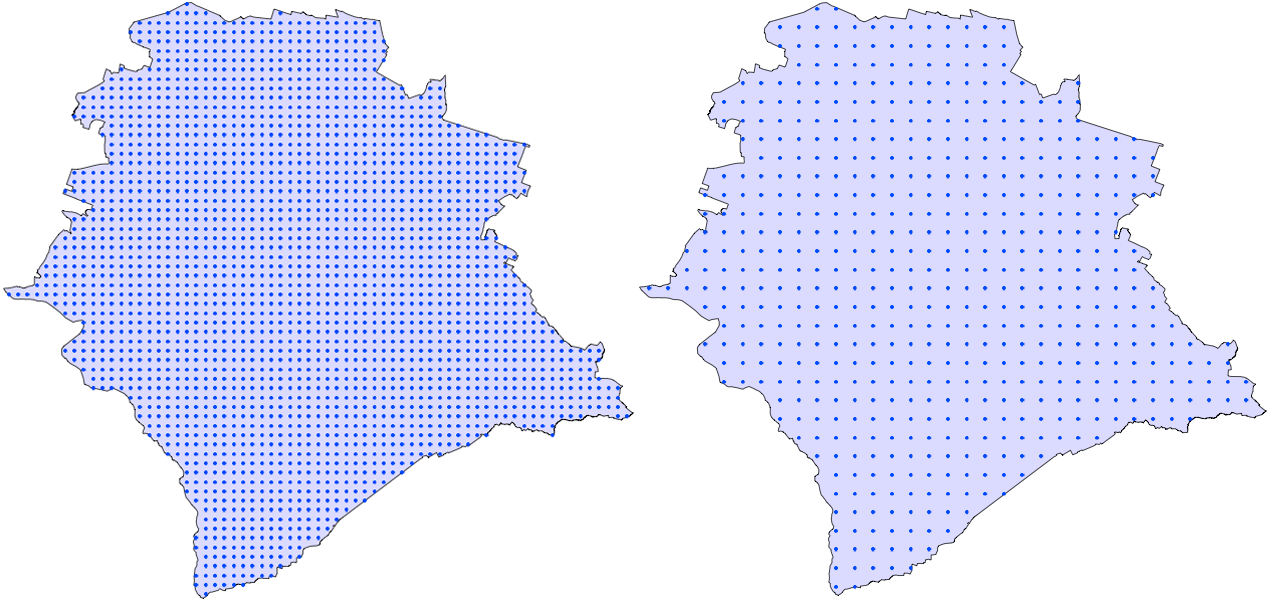
\includegraphics[width=\textwidth]{figures/matsim4urbansim/resolution.png}
\caption{The figure visualizes how the study area (blue area) is  subdivided into cells of configurable size by using the "cell\_size"  parameter. The left illustration has a side length of 200 meter  (cell\_size=200), the right illustration has a side length of 400 meter  (cell\_size=400). The blue dots are the corresponding cell centroids,  which serve as measuring points for the accessibility computation.}
\end{figure}

\begin{itemize}
	\item \textbf{accessibility\_parameter}: At this point the marginal utilities e.g. for different transport modes can be configured (\sout{for calibration instructions see \href{http://www.matsim.org/node/650}{here}} no this has nothing to do with calibration. kn, apr'13]]):   
\begin{itemize}
	\item \textbf{accessibility\_destination\_sampling\_rate}: This  determines the percentage of considered opportunities, currently work  places, for the accessibility computation. A value of 1 is recommended.
	\item \textbf{use\_MATSim\_parameter}: Enables MATSim default settings for the following parameter:     
\begin{itemize}
	\item \textbf{use\_logit\_scale\_parameter\_from\_MATSim}: This sets the logit scale parameter to a MATSim default value (currently this is 1.0)
	\item \textbf{use\_car\_parameter\_from\_MATSim}: This sets the marginal utility for traveling by car (beta$_tt,car$) to a MATSim default value (currently -12 utils/h). Otherwise the car\_parameter settings (see below) are used.
	\item \textbf{use\_walk\_parameter\_from\_MATSim}: This sets the marginal utility for traveling on foot (beta$_tt,walk$) to a MATSim default value (currently -12 utils/h). Otherwise the walk\_parameter settings (see below) are used.
	\item \textbf{use\_raw\_sums\_without\_ln}: If enabeld the summation of the term exp(V$_ik$) is computed, i.e.accessibility is computed as A$_i$:=sum$_k$( exp(V$_ik$) ) for all opportunities k.
\end{itemize}
	\item \sout{\textbf{logit\_scale\_parameter}: Set a custom value for the logit scale parameter. Make sure that "use\_logit\_scale\_parameter\_from\_MATSim" is disabled!}


((this functionality is currently disabled. It is not clear if the  following parameters should refer to the best path computed by matsim  (according to a different utility function), or if they should compute a  new best path according to that new utility function (where, however,  congested would not be equilibrated). kn, apr'13)) 

\sout{\textbf{car\_parameter} and \textbf{walk\_parameter}}: This allows to configure the disutility of traveling V$_ik,mode$ for a given mode (car, bicycle, walk) and thus to configure the accessibility measurement. V$_ik,mode$ is composed as follows:

%%V$_ik,mode$:= V$_ik,tt,mode$ + V$_ik,tt$^2$mode$ + V$_ik,ln(tt),mode$ + V$_ik,td,mode$ + V$_ik,td$^2$mode$ + V$_ik,ln(td),mode$ + V$_ik,m,mode$ + V$_ik,m$^2$mode$ + V$_ik,ln(m),mode$

     where "tt" are travel times, "td" are travel distances and "m" are monetary costs.

     Each summand $V_ik,xx,mode$ consists of the following contributions, see Figure 5:
\begin{enumerate}
	\item \sout{The disutility of travel of reaching the transport network from origin \emph{i}. It is assumed that opprotunities (e.g. work places) can only be reached via the transport network.}
	\item \sout{The disutiliy of travel on the network towards opportunity \emph{k}}
	\item \sout{The disutility of travel reaching opportunity \emph{k} from the transport network}
\end{enumerate}
\end{itemize}
\end{itemize}

\sout{As a result the disutility V$_ik,xx,mode$ is composed as follows:}

\sout{V$_ik,xx,mode$:= beta$_xx,wlk$* xx$_wlk,gap,i $+ beta$_xx,mode$ * XX$_mode$ + beta$_xx,wlk$ * xx$_wlk,gap,k$
\\
\\  where xx refers to the travel costs (tt, tt$^2$,ln(tt), td, td$^2$,ln(td), m, m$^2$,ln(m)) and beta$_xx,wlk$ and beta,$_xx,mode $are marginal utilities that convert the given travel cost into utils.
\\
\\  Setting the marginal utility beta$_xx$ to zero removes the corresponding summand from the equation. In order to use your own V$_ik,mode$  make sure that the corresponding switches  ("use\_car\_parameter\_from\_MATSim" and/or  "use\_walk\_parameter\_from\_MATSim") are disabled.}

\begin{figure}[htp]
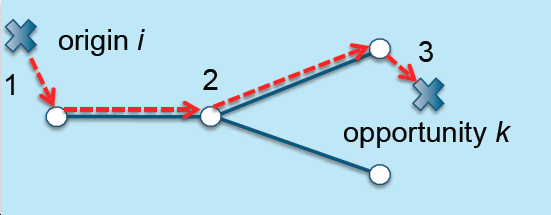
\includegraphics[width=.5\textwidth]{figures/matsim4urbansim/vik.png}
\caption{The composition of the disutility V$_ik,xx,mode $consists  of three parts: the cost (1) to reach network from i, (2) the cost on  the network and (3) the costs to reach the opportunity \emph{k} from the network.}
\end{figure}

\begin{itemize}
	\item \textbf{random\_location\_distribution\_radius\_for urbansim\_zone}:  This option is only relevant for UrbanSim zone applications. It  randomly distributes persons living in a certain zone within a given  radius (in meter) around the zone centroid. See also section 4  "Additional MATSim4UrbanSim Parameters" for an alternative distribution  of persons.
\end{itemize}

\begin{figure}[htp]
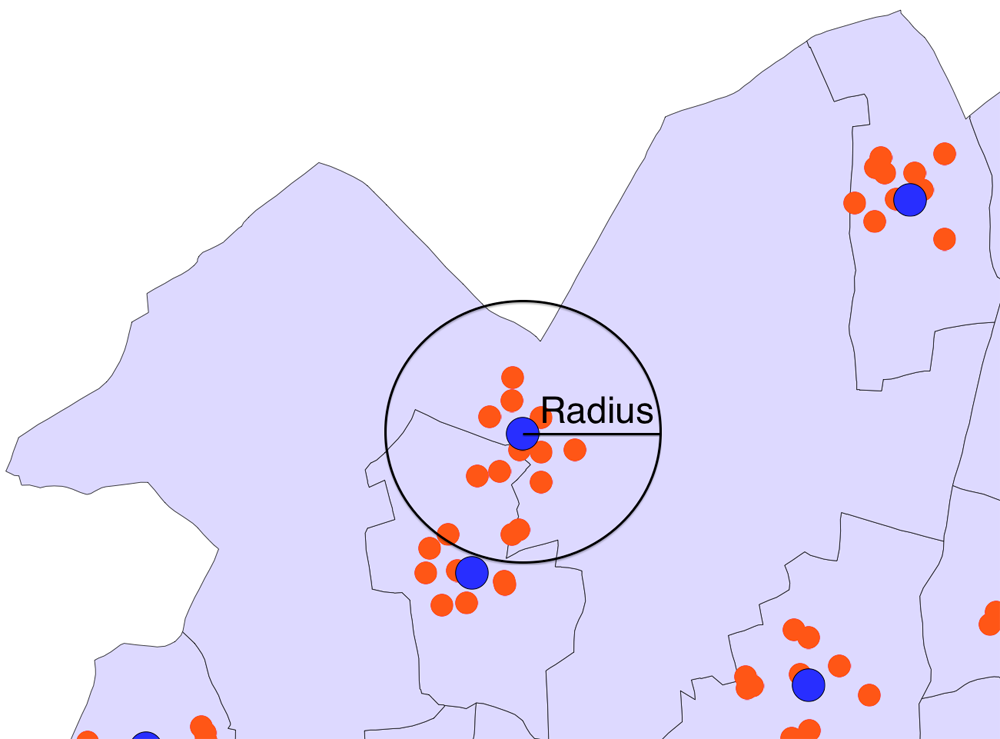
\includegraphics[width=\textwidth]{figures/matsim4urbansim/radius.png}
\caption{The random\_location\_distribution\_radius\_ for\_urbansim\_zone  parameter randomly distributes persons (red dots) living in a certain  zone within a given radius around the zone centroid (blue dot).}
\end{figure}


\textbf{MATSim Config}:

Thissectioncontainsparametersfor theconfigurationof thetrafficmodel.
\begin{itemize}
	\item \textbf{common}: The common subsection provides some basic configuration options for MATSim   
\begin{itemize}
	\item \textbf{external\_MATSim\_config}: This allowsto integratean external MATSim configuration for a specified UrbanSim year by setting the relative path to the separate configuration file, which must be located in the OPUS HOME directory.
\\Note  that overlapping parameter settings are overwritten by the external  configuration such as the population sampling rate, network, last  iteration, input plans file, plan calc score and strategy parameters (if  defined in both, the MATSim4UrbanSim and external MATSim config).
\\     Previously, parameter settings made in the external conguration were overwritten.
\\
\\     In order to set an external configuration file add the following  lines in the "travel\_model\_configuration $>$ matsim\_config $>$ common"  section:
\\
\begin{verbatim}
<external_matsim_config type="dictionary">
  <matsim_config name="2001" type="file">relative_path/to/external_matsim_config.xml</matsim_config>
</external_matsim_config>}
\end{verbatim}
	\item \textbf{matsim\_network\_file}: This points, as the name  implies, to a road network in MATSim format. A relative path (located in  the OPUS\_HOME directory) to the network file is expected.
	\item \textbf{last\_iteration}: This gives the number of MATSim iterations to perform. In MATSim iterations start at zero.
	\item \textbf{input\_start\_plans\_file}: This gives the path to a  “relaxed” plans file from which MATSim starts ("warm start"). It allows  MATSim to recycle agent decisions like route and departure times from a  previous run to speed up computing time. If this is not set, MATSim  will construct its initial plans file purely from UrbanSim input, and  take much longer to relax ("cold start"). See below (section 5) how to  create a plans file.
	\item \textbf{hot\_start\_plans\_file}: To speed up computing  times for traffic simulation it would be desireable to reuse the output  plans file of one MATSim run for one UbanSim year as input for a MATSim  run of a following UrbanSim year. This describes "hot start" (as opposed  to "warm start") in MATSim. At this point one can specify a location  where MATSim should store the plans file. If no location is  provided but an "input\_start\_plans\_file" is given MATSim has "warm  start", otherwise MATSim has a "cold start".
	\item \textbf{backup}: If enabled the following files are saved  after each MATSim run: the MATSim configuration, the final plans file,  the MATSim input files for UrbanSim and some output files to visualize  accessibility via R. These files are stored using the follwing folder  structure: OPUS\_HOME/matsim4opus/backup/runXXXX, where XXXX refers to  the current UrbanSim simulation year.
\end{itemize}
	\item \textbf{plan\_calc\_score}: This specifies the following activity constraints:   
\begin{itemize}
	\item \textbf{home\_activity\_typical\_duration}: Typical home activity duration (in seconds)
	\item \textbf{work\_activity\_typical\_duration}: Typical work activity duration (in seconds)
	\item \textbf{work\_activity\_opening\_time}: The earliest time where a work activity can be started (in seconds)in seconds
	\item \textbf{work\_activity\_latest\_start\_time}: The latest time to start a work activity (in seconds)
\end{itemize}
	\item \textbf{strategy}:   
\begin{itemize}
	\item \textbf{max\_agent\_plan\_memory\_size}: This gives the number of plans per agent, where 0 means infinity. A plans size of 5 is recommended.
	\item \textbf{time\_allocation\_mutator\_probability}: Probability$^*$ thatan agent obtains new activity starting and end times
	\item \textbf{reroute\_dijkstra\_probability}: Probability$^*$ that an agent obtains a new route
	\item \textbf{change\_exp\_beta}\textbf{\_probability}: Probability$^*$ that an agent switches between existing plans
\end{itemize}
\end{itemize}

*) despite its name, this really is a "weight"

\textbf{Years\_To\_Run}:

This defines the years in which the travel model should run. In order  to add additional years add the following lines in the  "travel\_model\_configuration $>$ years\_to\_run" section:
\begin{verbatim}

<run_description type="directory">
    <year type="integer">2002</year>
</run_description>
\end{verbatim}

\subsubsection{4 Additional MATSim4UrbanSim Parameters}

Some MATSim4UrbanSim configuration parameters are only availabe via the standard MATSim configuration, see Figure 7. A sample MATSim configuration containing olny these relevantparameters forMATSim4UrbanSim can be downloaded \href{https://svn.vsp.tu-berlin.de/repos/public-svn/matsim/examples/countries/us/seattle/external_matsim_config_with_matsim4urbansim_settings.xml}{here}. The following modules and parameters are available:

\textbf{MATSim4UrbanSimParameter}:

This module provides the following parameter:
\begin{itemize}
	\item \textbf{timeOfDay}: Specify the time of day (in seconds)  for which the zone2zone impedance matrix and accessibilites should be  calculated be calculated. By default this is set to 8am (28800 sec).
	\item \textbf{urbanSimZoneShapefileLocationDistribution}: This  option is only relevant for UrbanSim zone applications. This randomly  distributes persons living in a certain zone within the zone boundaries  provided by zone shape file, see Figure 8. Enter the path to a zones  shape file here. Note: This deactivates random\_location\_distribution\_radius\_for urbansim\_zone (see above).
	\item \textbf{usePtStops}: This is a switch to enable a  MATSim4UrbanSim specific pseudo pt based on a given csv input file  provided at the 'ptStops' parameter (see next).
	\item \textbf{ptStops}: This parameter expects a csv input file  providing a pt stop id and a x and y coordinate. The csv files needs a  header indicating the cooresponding columns by "id" (for the pt stop  id), "x" and "y" for the coordinates. A sample file to illustrate the  format can be found \href{https://svn.vsp.tu-berlin.de/repos/public-svn/matsim/examples/countries/us/seattle/ptStops.csv}{here}.
	\item \textbf{useTravelTimesAndDistances}: This is a switch to  initialize the MASim4UrbanSim specific pseudo pt by the given pt travel  times and distances provided at the parameters 'ptTravelTimes' and  'ptTravelDistances' (see next). This requires the 'usePtStops' to be TRUE and a ptStop input file provided at 'ptStops' parameter.
	\item \textbf{ptTravelTimes}: This parameter expects an input  file providing an origin and destination ptStop id, which is consistent  with the ptStop id provided at 'ptStops', and the corrosponding travel  time in minutes. The input file can be in VISUM format (e.g. *.JRT) or  just a text file (*.txt) with space separated values in the following  order: origin ptStop id, destination ptStop id and travel times in  minutes. A sample file illustrating format can be found \href{https://svn.vsp.tu-berlin.de/repos/public-svn/matsim/examples/countries/us/seattle/sampleTravelTimes.jrt}{here}.
	\item \textbf{ptTravelDistances}: This parameter expects an input  file providing an origin and destination ptStop id, which is consistent  with the ptStop id provided at 'ptStops', and the corrosponding travel  distances in meter. The input file can be in VISUM format (e.g. *.JRD)  or just a text file (*.txt) with space separated values in the following  order: origin ptStop id, destination ptStop id and travel distances in  meter. A sample file illustrating format can be found \href{https://svn.vsp.tu-berlin.de/repos/public-svn/matsim/examples/countries/us/seattle/sampleTravelTimes.jrt}{here}.
\end{itemize}

%%\textbf{Please do not use the following parameter anymore}.  It was decided to disable the custom parameter settings for the beta  values. This concerns the beta parameters in the UrbanSim GUI (car and  walk) and the external MATSim config file (bike and pt).
%%\begin{itemize}
%%	\item \sout{\textbf{betaBikeXXX parameter}: This allows to  configure the disutility of traveling for travelling by bicycle. For  more information see ``car\_parameter and walk\_parameter'' above\textbf{. }}
%%	\item \sout{\textbf{betaPtXXX parameter}: This allows to  configure the disutility of traveling for travelling by pseudo pt. For  more information see ``car\_parameter and walk\_parameter'' above\textbf{.}}
%%\end{itemize}

\textbf{ChangeLegMode and Strategy}:

A full description for the changeLegMode module is given \href{http://www.matsim.org/node/387}{here}.  Basically the changeLegMode module defines the transport modes that can  be used by MATSim agents. Currently MATSim4UrbanSim supports car, pt,  bike (bicycle) and walk. In order to allow MATSim agents to switch  between these modes either the "ChangeLegMode" or "ChangeSingleLegMode"  module must be set in the strategy module, a comprehensive description  is given \href{http://www.matsim.org/node/617}{here}.

Note: When using MATSim4UrbanSim  make sure that any strategy defined in the standard MATSim  configuration has an "index" $>$= 4 (ModuleProbability\_index,  Module\_index). Otherwise these strategies are overwritten by the  strategies that are configurable via the OPUS GUI, see above "strategy".

\begin{figure}[htp]
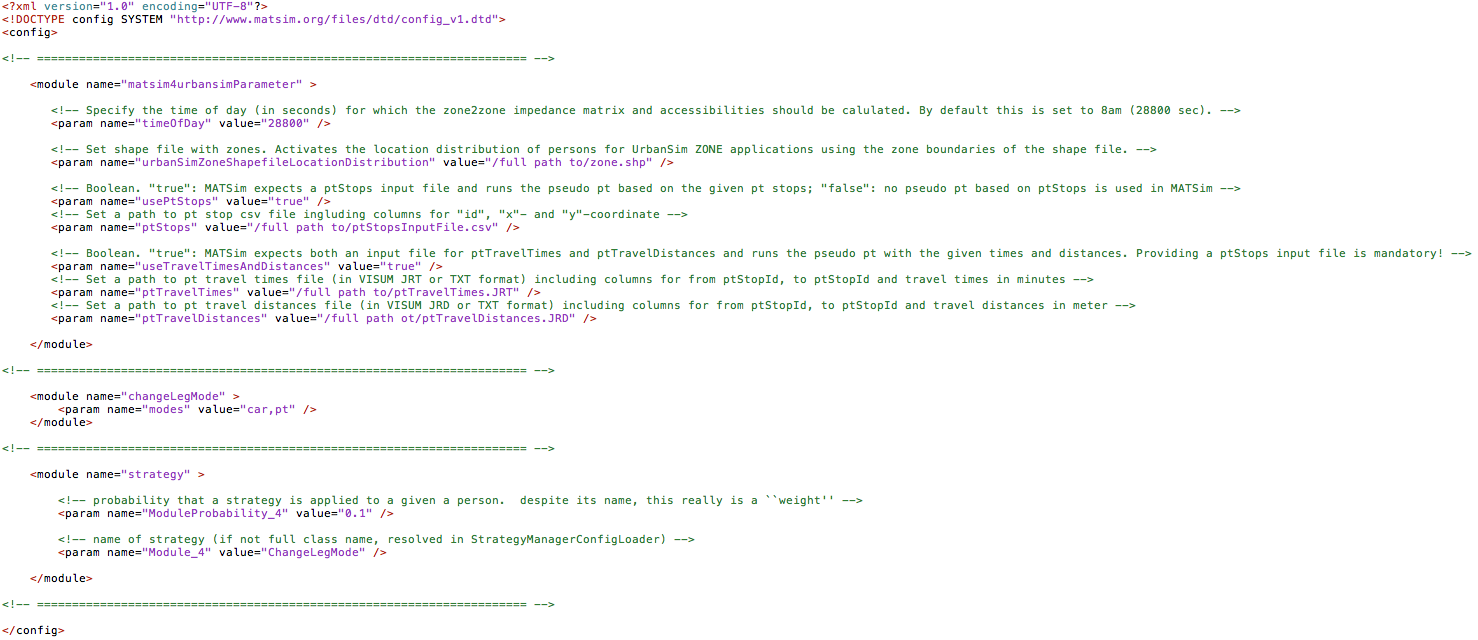
\includegraphics[width=\textwidth]{figures/matsim4urbansim/external_matsim_config_1.png}
\caption{Some addidional configuration settings for MATSim4UrbanSim  are only available/configurable via the standard MATSim configuration,  which are depicted in this illustration.}
\end{figure}

\begin{figure}[htp]
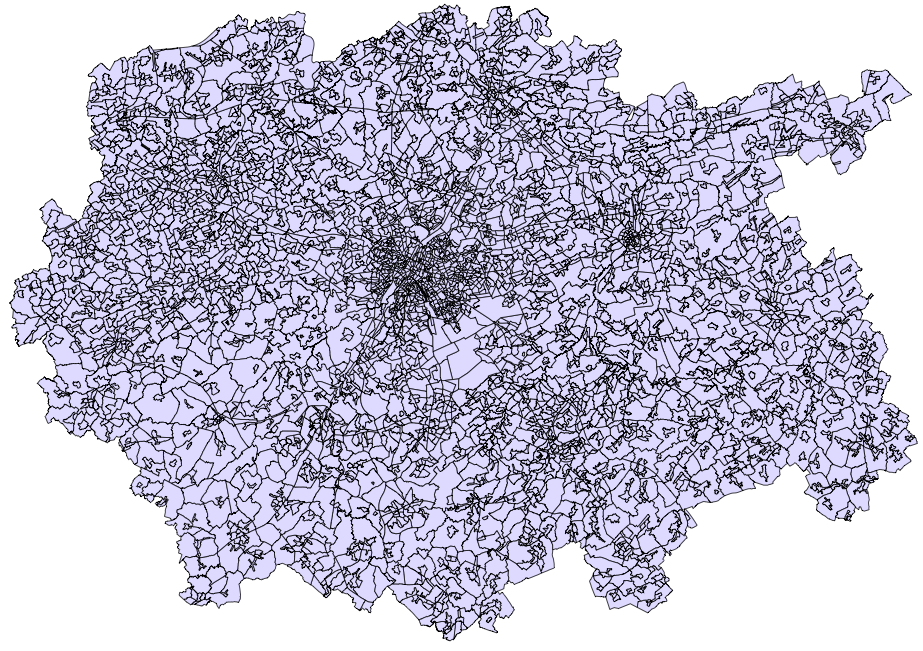
\includegraphics[width=\textwidth]{figures/matsim4urbansim/brussel_zone_shapefile.png}
\caption{A zone shape file at the example of the greater Brussels area.}
\end{figure}

\subsubsection{5 Create An Initial Plans File}

This section describes how to generate an initial plans file for warm  start. This example based on the Seattle parcel configuration, which  can be downloaded in section 3.
\begin{enumerate}
	\item Launch the OPUS GUI and open the sample Seattle parcel configuration.
	\item Switch to the Models tab and set the last iteration to 100" or higher
	\item Note: Leaving the population sample rate at 0.01 will generate a 1\% plans file
	\item Switch to the Scenarios tab and right-click on "Seattle\_baseline" and then on "Run this Scenario" to start the simulation
	\item When the simulation finished find the plans file at  "OPUS\_HOME/matsim4opus/output/ITERS/it.100/100.plans.xml.gz" and move it  to a convenient place, e.g. into  "OPUS\_HOME/data/seattle\_parcel/base\_year\_data/2000/matsim/plans"
	\item Finally enter the relative path to the plans-file, i.e.  data/seattle\_parcel/base\_year\_data/2000/matsim/plans/100.plans.xml.gz,  into the \textbf{input\_start\_plans\_file }field in the OPUS GUI  under "travel model conguration $>$ matsim\_config $>$ common" to start  MATSim in warm start mode next time.
\end{enumerate}

\subsubsection{6 Travel Model Visualization}

There are at least two options to visualize the traffic in MATSim see \href{http://matsim.org/node/741}{here}.

\subsubsection{7 Limitations}

The Java virtual machine (VM) can't allocate more than 1.5 GB on  32bit Windows systems, no matter how much RAM is available in your  computer. For this reason the travel model plug-in runs MATSim with 1.5  GB on Windows (32bit and 64bit) and with 4 GB on Mac and Linux systems  by default. This may cause longer computing times on Windows  computers.

%%\vfill\eject
%%\subsection{MATSim4UrbanSim (Frist Release)}

%%\subsubsection{The current user guide can be found \href{http://matsim.org/docs/extensions/matism4urbansim}{here} !!!}



%%\subsubsection{Guide on UrbanSim usage of the travel model plug-in}

%%The current travel model plug-in implementation is applicable for  PSRC (Puget Sound Region Council) parcel, Seattle parcel and Zurich  parcel scenario.

%%Note that some of the instructions may change since the travel model plug-in is still under development.

%%\subsubsection{1 Prerequisites}

%%You must have installed UrbanSim, before getting started with the  travel model plug-in. The following provides an entry point to install  UrbanSim and continues with installation instructions for additional  software packages required by the travel model plug-in.

%%\subparagraph{Hints for installing UrbanSim}

%%To install UrbanSim please follow the UrbanSim Downloads and Installation Instructions on \href{http://urbansim.org/Download/}{http://urbansim.org/Download/}.

%%When installing OPUS and UrbanSim manually (Windows users may require  an additional svn client, e. g. totoisesvn, which is available for free  at \href{http://tortoisesvn.tigris.org/}{http://tortoisesvn.tigris.org/})  please make sure to get the source code for the stable release or the  latest development version as described in Downloading Sample Data and  Source Code on: \href{http://urbansim.org/Download/DownloadingSampleDataAndSourceCode}{http://urbansim.org/Download/DownloadingSampleDataAndSourceCode}.

%%Windows users using the installer are getting the source code and data automatically.

%%Finally make sure that all UrbanSim environment variables, meaning  OPUS\_HOME, OPUS\_DATA\_PATH and PYTHONPATH, are set as described in the  installation instructions, see \href{http://urbansim.org/Download/SixtyFourBitMachines}{http://urbansim.org/Download/SixtyFourBitMachines} for Windows, \href{http://urbansim.org/Download/MacintoshInstallation}{http://urbansim.org/Download/MacintoshInstallation} for Mac or \href{http://urbansim.org/Download/LinuxInstallation}{http://urbansim.org/Download/LinuxInstallation} for Linux.

%%Note:  For using the travel model plug-in it is sufficient only to install the  required Python packages, i. e. numpy, scipy, lxml, sqlalchemy and  elixir.

%%\subparagraph{MATSim4UrbanSim prerequisites}

%%In addition to the UrbanSim installation the MATSim travel model plug-in requires the following software installed:
%%\begin{itemize}
%%	\item Java JDK 1.6 or newer: Download and install the newest version  of the Java SE Development Kit (JDK) for your operating system from \href{http://www.oracle.com/technetwork/java/javase/downloads/index.html}{http://www.oracle.com/technetwork/java/javase/downloads/index.html}. Make sure adding Java's /bin directory to the PATH environment variable. Click\href{http://java.com/en/download/testjava.jsp}{here}to test ifjavaisalready installed on your computer.
%%	\item Python XML Schema Bindings (PyXB): Download the PyXB distribution file from \href{http://sourceforge.net/projects/pyxb/}{http://sourceforge.net/projects/pyxb/} and extract it to a convenient place. Windows users may use Win-Rar to extract tar or gz files, which is available for free at \href{http://www.win-rar.com/}{www.win-rar.com}.
%%\\
%%\\   Open a command prompt (Windows) or a terminal (Mac, Linux). To install  PyXB (this may requires administrator or root privileges) go into  the extracted directory and type
%%\\


%%\texttt{python setup.py install}
%%\end{itemize}

%%\subsubsection{2 MATSim4UrbanSim installation}

%%This section describes how to install MATSim4UrbanSim.

%%\subparagraph{Automatic installation}

%%Make sure to have the Python lib directory included to the  PYTHONPATH. This is the directory that contains the site-package  directory that is already included in the PYTHONPATH. The lib directory  should be something like


%%\texttt{C:$\backslash$Python2.6$\backslash$Lib$\backslash$ }for Windows,


%%\texttt{/Library/Frameworks/Python.framework/Versions/2.6/lib/} for Mac or


%%\texttt{/usr/lib/python2.6/} for Linux (Ubuntu).

%%To install MATSim4UrbanSim open command prompt (Windows) or a  terminal (Mac, Linux) and navigate to opus\_matsim/configs in the opus  source directory. Than type


%%\texttt{python install\_matsim4urbansim.py}

%%This creates the subdirectories matsim4opus/jar, loads required  MATSim executables and libraries and configures them. After the  installation the file/directory structure should look something like  Figure 1.

%%To test whether the MATSim4UrbanSim installation was successful follow the instructions described in Section 2.3.

%%Note: The installer will replace jar-files and libraries from a previous MATSim4UrbanSim installation.

%%\subparagraph{Manual installation}

%%In case that the automatic installation does not work follow these instructions:
%%\begin{itemize}
%%	\item Create the following directory structure in OPUS\_HOME: OPUS\_HOME/matsim4opus/jar
%%	\item Download the following files from \href{http://www.matsim.org/files/builds/}{http://www.matsim.org/files/builds/} into the jar directory:   
%%\begin{itemize}
%%	\item MATSim\_rXXXXX.jar (where XXXXX refers the current revision)
%%	\item MATSim\_libs.zip
%%	\item matsim4urbansim-X.X.X-SNAPSHOT-rXXXXX.zip (where XXXXX refers the current revision)
%%\end{itemize}
%%	\item Rename MATSim\_rXXXXX.jar into "matsim.jar".
%%	\item Extract the zip files MATSim\_libs.zip and matsim4urbansim-X.X.X-SNAPSHOT-rXXXXX.zip. After that the zip files can be removed.
%%	\item Rename the directory matsim4urbansim-X.X.X-SNAPSHOT-rXXXXX into  "contrib". Than navigate into contrib and rename the jar-file  matsim4urbansim-X.X.X-SNAPSHOT.jar into "matsim4urbansim.jar".
%%\end{itemize}

%%Be careful when renaming files or directories (i. e. make sure  that everything is written in lower case and check for spelling errors).  After the installation the file/directory structure in the matsim4opus  directory should look something like Figure 1. To test whether the  MATSim4UrbanSim installation was successful follow the instructions  described in Section 2.3.

%%\subparagraph{Test your MATSim4UrbanSim installation}

%%To test your installation open a command prompt (Windows) or a  terminal (Mac, Linux) and navigate to opus\_matsim/tests in the opus  source directory (PYTHONPATH). Then type


%%\texttt{python travel\_model\_test.py}

%%This starts a test scenario. If the test completes without errors, your travel model plug-in should be working.


%%%\includegraphics{User%27s%20Guide_files/structure.png}Figure 1: After the installation the matsim4opus directory should contain the depicted files and subdirectories.

%%\subsubsection{3 Using MATSim for UrbanSim}

%%This section aims to explain the MATSim travel model plug-in at the example of the Seattle\_parcel scenario.\textbf{ In order to run Seattle parcel with MATSim the following steps are necessary:} Download the\href{https://svn.vsp.tu-berlin.de/repos/public-svn/matsim/examples/countries/us/seattle/matsim.zip}{ matsim\_seattle.zip}  and unzip the file into your OPUS\_DATA/seattle\_parcel/base\_year/2000/  directory. After that your seattle\_parcel base year cache should look  like Figure 2. The zip-file contains a road network and a plans-file,  used by MATSim. Thesestepsalso apply for the PSRC scenario using\href{http://matsim.org/uploads/matsim_psrc.zip}{matsim\_psrc.zip} file.


%%%\includegraphics{User%27s%20Guide_files/seattle_parcel_base_year_dir.png}Figure  2: Put the unzipped "matsim" directory, including a road network and a  plans-file, into your seattle\_parcel base year cache in order to run  MATSim as a travel model for the Seattle\_parcel scenario.

%%In a recent effort the MATSim configuration is embedded into  UrbanSim. This enables the MATSim (travel model) plug-in in UrbanSim and  provides all necessary or basic options to run MATSim via the OPUS GUI.  To enable the MATSim plug-in requires the travel model configuration  section in the UrbanSim configuration as depicted in Figure 3.

%%Sample configurations, including the travel model configuration  section, can be found for the Seattle\_parcel (seattle\_parcel.xml) and  PSRC\_parcel (psrc\_parcel.xml) scenario in the opus source directory at  opus\_matsim/configs.

%%Windowsuserswill need to replaceslashesinpathsbybackslashes, e.g. replace "data/seattle\_parcel/base\_year\_data/2000/matsim/network/psrc.xml.gz" by "data$\backslash$seattle\_parcel$\backslash$base\_year\_data$\backslash$2000$\backslash$matsim$\backslash$network$\backslash$psrc.xml.gz".


%%%\includegraphics{User%27s%20Guide_files/configuration.png}Figure  3: Adding the travel\_model\_configuration section into an UrbanSim  configuration enables the MATSim plug-in and configuration options  within OPUS GUI.

%%\subparagraph{Travel Model configuration options}

%%This sections explains step by step the MATSim configuration options provided by the travel model plug-in.

%%Launch the OPUS GUI and open the Seattle\_parcel sample configuration  located at opus\_matsim/config/seattle\_parcel.xml in opus source  directory. Switch to the Models tab to get to the travel model  configuration section as shown in Figure 4. The following options are  available:
%%\begin{itemize}
%%	\item \textbf{Models}: The models section contains three models integrating MATSim into UrbanSim:   
%%\begin{itemize}
%%	\item Get\_cache\_data\_into\_matsim generates input data for MATSim and stores it a specified location.
%%	\item Run\_travel\_model executes MATSim.
%%	\item Get\_matsim\_data\_into\_cache imports the results of the traffic simulation for the next UrbanSim iteration.
%%	\item By default all models are enabled. Only disable models if you know what you are doing.
%%\end{itemize}
%%\end{itemize}
%%\begin{itemize}
%%	\item \textbf{MATSim4UrbanSim}: This section contains options concerning the interaction of both simulation models MATSim and UrbanSim.   
%%\begin{itemize}
%%	\item The sampling\_rate determines the percentage of considered  travellers for a MATSim run. 0.01 means that only one percent of  travelers are considered for the traffic simulation. This option allows  to speed up computations on the MATSim side, e. g. during testing a  scenario.
%%	\item Note that low sampling rates cause some peculiarities in terms of  realism. In this situation results are useful for sketch planning only,  not for quantitative analysis. Higher sampling rates need more ram and  hard drive space.
%%\end{itemize}
%%	\item \textbf{MATSim Config}: The common subsection provides some basic configuration option for MATSim.   
%%\begin{itemize}
%%	\item The matsim\_network\_file points, as the name implies, to a road  network in MATSim format. This expects a relative path to the network  file located in the OPUS\_HOME directory.
%%	\item Determine the number of MATSim iterations with the item last iteration. In MATSim iterations start at zero.
%%\end{itemize}
%%\end{itemize}
%%\begin{itemize}
%%	\item \textbf{Years\_To\_Run}: This defines the years in which the travel model should run.
%%\\
%%\\   Adding additional years requires to edit the configuration file  directly, e. g. with a xml editor, within the year\_to\_run section in the  travel\_model\_configuration. Make sure that each year you are adding is  surrounded by the run\_description tags like this:
%%\end{itemize}


%%\texttt{ $<$run\_description type="directory"$>$}


%%\texttt{  $<$year type="integer"$>$2002$<$/year$>$}


%%\texttt{ $<$/run\_description$>$}

%%All configuration options can be easily edited in the OPUS GUI by clicking on the value or check box on the right hand side.


%%%\includegraphics{User%27s%20Guide_files/opus_gui.png}Figure 4: Configuring MATSim via the travel model configuration section in OPUS GUI.

%%\subsubsection{4 Travel Model Visualization}

%%There are at least two options to visualize the traffic in MATSim:
%%\begin{enumerate}
%%	\item \href{http://matsim.org/docs/extensions/otfvis}{OTFVis}
%%	\item \href{http://senozon.com/products/via}{Senozon via}
%%\end{enumerate}

%%\subsubsection{5 Limitations}

%%\subsubsection{The Java virtual machine (VM) can't allocate more  than 1.5 GB on Windows systems, no matter how much RAM is available in  your computer. For this reason the travel model plug-in runs MATSim with  1.5 GB on Windows and with 2 GB on Mac and Linux systems by default.  This may cause longer computing times on Windows computers.}

%%\vfill\eject
\subsection{The MATSim network for the Brussels application}

\subsubsection{Note:}

The current MATSim network for the Brussels case study can be downloaded \href{https://svn.vsp.tu-berlin.de/repos/public-svn/matsim/examples/countries/be/brussels/network/belgium_incl_borderArea_hierarchylayer4_clean_simple.xml.gz}{here}! In the following it is described step by step how this network is created by using Open Street Map (OSM).

\subsubsection{Step 1:}

The network for the Brussels case study is composed of separate OSM  networks for Belgium and its bordering regions in the Netherlands,  Germany, Luxembourg and France. The following OSM files are used, which  are available at \href{http://download.geofabrik.de/osm/europe/}{http://download.geofabrik.de/osm/europe/}:
\begin{itemize}
	\item  alsace.osm.bz2
	\item  belgium.osm.bz2
	\item  champagne-ardenne.osm.bz2
	\item  lorraine.osm.bz2
	\item  luxembourg.osm.bz2
	\item  netherlands.osm.bz2
	\item  nord-pas-de-calais.osm.bz2
	\item  nordrhein-westfalen.osm.bz2
	\item  picardie.osm.bz2
	\item  rheinland-pfalz.osm.bz2
	\item  saarland.osm.bz2
\end{itemize}

\subsubsection{Step 2:}

These OSM files are now merged to a coherent OSM network in a two  step process using the java command line application Osmosis. A deteiled  manual for Osmosis can be found at \href{http://wiki.openstreetmap.org/wiki/Osmosis}{http://wiki.openstreetmap.org/wiki/Osmosis}.
\begin{itemize}
	\item In the first step each OSM network is treated separately on the command line as follows:
\end{itemize}
\begin{verbatim}
osmosis --rx xxx.osm.bz2 --lp interval=60 --bb top=51.671 left=2.177 \
    bottom=49.402 right=6.764 completeWays=yes --tf accept-ways \
    highway= motorway,motorway_link,trunk,trunk_link,primary,primary_link,secondary,\
    tertiary,minor,unclassified,residential,living_street --tf reject-relations \
    --used-node --wx xxx_filtered.osm.bz2
\end{verbatim}

This modifies each network file as follows:
\begin{itemize}
	\item The network links and nodes that are  located in the area of interest are extracted. This area, defined by a  rectangle containing Belgium and its bordering regions.
	\item Links and nodes that do not correspond  to one of the following road types in OSM, for instance links and nodes  belonging railways, are removed: motorway, trunk, primary, secondary,  tertiary, minor, unclassified, residential and living street.
\end{itemize}
\begin{itemize}
	\item In the second step, the modified networks are merged on the command line as follows:
\end{itemize}
\begin{verbatim}
osmosis --rx xxx_filtered.osm.bz2 --lp interval=30 --m --wx belgium_incl_borderArea.osm
\end{verbatim}

At this point we have one merged OSM network "belgium\_incl\_borderArea.osm" for our area of interest.

\subsubsection{Step 3:}

The merged OSM network is converted into MATSim format. To be  consistent with the UrbanSim coordinates in the Brussels case study the  MATSim default network coordinates are transformed using the \emph{Belge Lambert 72}  projection. One hierarchy level is used to avoid side effects of having  different network densities within and around the study area. The used  hierachy level includes, in OSM terms, links and nodes of secondary  roads or greater.

Finally the MATSim network is “cleaned” and “simplified”. Cleaning  means, that only links that can be reached by other links are kept in  the network. Simplifying means, that a set of links that belong to a  road are merged into one single link. The resulting network is depicted  below, where the study area is highlighted in blue.

The Java code for the conversion is given in here:
\begin{lstlisting}{language=Java}
Scenario sc = ScenarioUtils.createScenario(ConfigUtils.createConfig());
// creating an empty matsim network
Network network = sc.getNetwork();
// using the Belge Lambert 72 projection for the matsim network
CoordinateTransformation ct = TransformationFactory
        .getCoordinateTransformation(TransformationFactory.WGS84, "EPSG:31300");
OsmNetworkReader osmReader = new OsmNetworkReader(network, ct);

osmReader.setKeepPaths(false);
osmReader.setScaleMaxSpeed(true);

// this layer covers the whole area, Belgium and bordering areas
// including OSM secondary roads or greater
osmReader.setHierarchyLayer(51.671, 2.177, 49.402, 6.764, 4);

// converting the merged OSM network into matsim format
osmReader.parse(INFILE);
new NetworkWriter(network).write(OUTFILE);
// writing out a cleaned matsim network and loading it
// into the scenario
new NetworkCleaner().run(OUTFILE, OUTFILE.split(".xml")[0] + "_clean.xml.gz");
Scenario scenario = (ScenarioImpl) ScenarioUtils
        .createScenario(ConfigUtils.createConfig());
new MatsimNetworkReader(scenario).readFile(OUTFILE.split(".xml")[0] + "_clean.xml.gz");
network = (NetworkImpl) scenario.getNetwork();

// simplifying the cleaned network
NetworkSimplifier simplifier = new NetworkSimplifier();
Set<Integer> nodeTypess2merge = new HashSet<Integer>();
nodeTypess2merge.add(new Integer(4));
nodeTypess2merge.add(new Integer(5));
simplifier.setNodesToMerge(nodeTypess2merge);
simplifier.run(network);
new NetworkWriter(network).write(OUTFILE.split(".xml")[0] + "_clean_simple.xml.gz");
\end{lstlisting}




%\includegraphics{User%27s%20Guide_files/belgium_incl_borderArea_hierarchylayer4_clean_simple.png}


\vfill\eject
\NextFile{OTFVis.html}
\section{OTFVis}

OTFVis  is a visualizer for MATSim. It can be used to replay snapshots of  simulations, or run a simulation and interact with it. The visualizer  makes use of hardware acceleration (OpenGL) and is thus also suitable  for visualizing large scenarios. If you have problems running OTFVis,  make sure to \href{http://www.matsim.org/docs/extensions/otfvis/opengl}{check your Graphics Card is able to support OTFVis}.

\subsection{Download / Requirements}

To use OTFVis, you need MATSim as well as the OTFVis extension. The  OTFVis extension is not yet available as an official release, so the  following documentation will use a nightly build of it.
\begin{itemize}
	\item Download a current nightly build of MATSim, the MATSim libraries and OTFVis from our \href{http://www.matsim.org/files/builds}{nightly build download page}.
	\item Unzip the MATSim libs
	\item Unzip the OTFVis Extension
\end{itemize}

You should now have: the MATSim jar, the libs directory, and the otfvis directory next to each other.

\subsection{Starting the Visualizer}

The main class for the visualizer is 
\texttt{org.matsim.contrib.otfvis.OTFVis}. The different ways to start OTFVis will be described in more details below.

The visualizer may require a lot of memory, it is thus advised to start it with the corresponding Java options, e.g. with 500MB:
\begin{verbatim}
java -Xmx500m-cp MATSim.jar:otfvis/otfvis.jarorg.matsim.contrib.otfvis.OTFVis arguments
\end{verbatim}

If you're on Windows, use 
\texttt{;} instead of 
\texttt{:} to  separate the jar files from each other. Also, depending on the version  you downloaded, you might have to adapt the file and directory names a  little bit.  

\subsection{Creating snapshots (mvi-files) from Events}

Use the following arguments:
\begin{verbatim}
-convert event-file network-file mvi-file [snapshot-period]
\end{verbatim}

to record a snapshot of all vehicles' positions every snapshot-period  seconds, based on the events and network given in the corresponding  files.

Example call:
\begin{verbatim}
java -cp MATSim.jar:otfvis/otfvis.jarorg.matsim.contrib.otfvis.OTFVis -convert output/50.events.txt.gz input/network.xml.gz output/50.visualization.mvi 300


\end{verbatim}

This will create a snapshot of every 5th minute and store it in the file 
\texttt{output/50.visualization.mvi}.

\subsection{Displaying MATSim Visualization Snapshots (mvi-files)}

Just pass the file as first argument. Example call:
\begin{verbatim}
java -cp MATSim.jar:otfvis/otfvis.jarorg.matsim.contrib.otfvis.OTFVis output/0.visualization.mvi
\end{verbatim}

\subsection{Displaying TRANSIMS Vehicle files}

For reasons of backward compatibility, OTFVis can display vehicles  files traditionally generated by TRANSIMS. As the vehicle file does not  include any network information, the network must be passed as well.  Example call:
\begin{verbatim}
java -cp MATSim.jar:otfvis/otfvis.jarorg.matsim.contrib.otfvis.OTFVis output/0.T.veh input/network.xml.gz
\end{verbatim}

\subsection{Displaying MATSim Network files}

OTFVis can display just a network. This is useful when building a  scenario, and a network converted from other data must be inspected.  Example call:
\begin{verbatim}
java -cp MATSim.jar:otfvis/otfvis.jarorg.matsim.contrib.otfvis.OTFVis input/network.xml.gz
\end{verbatim}

(Note: Currently only available in Nightly Builds since revision r5821)

\subsection{Start Interactive Simulation}

OTFVis can directly start a simulation and visualize it in real time.  As in that case, all data (esp. the population) is loaded into memory,  interactive queries about agents and link states can be issued from the  visualizer. To start OTFVis in this interactive, live mode, just pass it  the config-file you would otherwise pass to the Controler:
\begin{verbatim}
java -cp MATSim.jar:otfvis/otfvis.jar org.matsim.contrib.otfvis.OTFVis input/config.xml
\end{verbatim}

Please note that this will require even more resources (memory, cpu-speed) than only running the simulation with the Controler.

\subsection{Running OTFVis from within a windows systems}

As shown by the \href{http://www.matsim.org/downloads/nightly}{Nightly Builds}  tutorial OTFVis and other classes can be run by using the command line  or a shell script respectively. As the Unix based way is already  described by the tutorial, this is about the windows user.

The windows command line call looks similiar to the Unix based one. Finally, you should end with something like that
\begin{verbatim}
java -Xmx1500m -cp MATSim.jar:otfvis/otfvis.jarorg.matsim.contrib.otfvis.OTFVis %*
\end{verbatim}

which can be saved as a *.bat file, e.g. otfvis.bat. Please note that  the example is based on the assumption that otfvis.bat is saved in the  same folder as the matsim.jar and the libs folder. The placeholder \%*  will be substitued by the parameters you've specified when calling  otfvis.bat from the command line, e.g.
\begin{verbatim}
otfvis.bat -convert event-file network-file mvi-file
\end{verbatim}

To call the OTFVis from any folder, put the otfvis.bat into your PATH environment.

If your are more familiar with the point and click behaviour of win  systems, you can create a shortcut pointing to your otfvis.bat.
\begin{enumerate}

	\item By putting it on your desktop, you can drop any file on it, to call OTFVis with the file dropped, e.g. a network.

	\item 
Move  the shortcut to your SendTo folder and rename it to something like  OTFVis.lnk. Depending on the system you use, the SendTo folder should be  located in your home directory. Now you can start the OTFVis by  rightclicking at any file within your system, e.g. rightclick a  mvi-file, from the context menu select SendTo -$>$ OTFVis.

%\includegraphics{User%27s%20Guide_files/moz-screenshot.jpg}

\end{enumerate}



\vfill\eject
\subsection{OpenGL Requirements}

For  the hardware acceleration to work, (i) the OpenGL graphic card driver  installed on your machine must be at least of version 2.0 and (ii)  native libraries are required, which must be correctly set up.

\subsubsection{Check and Update Graphic Card Driver}

Either you use check and update mechanims / software already  installed (e.g. NVIDIA software, ATI update manager, etc...) or download  and install \href{http://www.realtech-vr.com/glview}{OpenGL Extension Viewer}.  After starting this little tool, it show all necessary information  abour your graphic card including OpenGL version. Please be sure that at  least \textbf{OpenGL version 2.0} is installed. Otherwise try  to find approriate driver updates of your graphic card (the read circles  in the Figure below shows the important featrues / information).


%\includegraphics{User%27s%20Guide_files/openglextensionviewer_png_4b5038ca1c.html}


\vfill\eject
\NextFile{TransEnergySim.html}
\section{Transportation Energy Simulation Framework (transEnergySim)}

\subsection{[module is still under construction]}

In this MATSim contribution a framework to simulate a whole range  oftranportation related energy scenarios is implemented. The focus  is on electric and plug-in hybrid electric vehicles. This contributio  is being built and updated as part of the PhD ofRashid A. Waraich  (waraich at ivt.baug.ethz.ch). As this is an open source project, which  encourages contribution by others, there are also modules, which have  been contriubted by the following people: Dr. Matthias D. Galus, Gil  Georges ?, Marina ?, Zain?, Raffaela?, etc.?


The following modules should be available soon/ are planned:
\begin{itemize}
	\item Inductive charging along roads
	\item Charging at activity location
	\item Several charging schemes including smart charging ("smart grid")
	\item V2G
	\item General energy flow model
	\item buy/sell of electricity price over market
\end{itemize}

These features require several basic constructs, which willalso be documented soon here:
\begin{itemize}
	\item vehicle fleet definition model
	\item vehicle energy consumption model
	\item charging infrastructure definition model
	\item output modules
	\item more to come here...
\end{itemize}

If you want to contribute with a new module to the framework  (e.g. for charging, energy consumption, emissions, etc.), please contact  Rashid A. Waraich (waraich at ivt.baug.ethz.ch).

\subsection{Applications}

TODO: Describe ARTEMIS and THELMA project here with figures and references.



TODO: also add work of stella, zain, raffaela, marina, etc. here.

\subsection{Emissions}

Modules for green house gas and other emissions coming soon here.

\subsection{Hints and Pitfalls}

ParallelEventHandling

Many of the modules for keeping track of charging and energy  consumption are based on event handlers. In order to avoid  raceconditions and accessing the same data unsynchronized (e.g. vehicle  trying to charge before the energy consumption is updated), we advise to  use the EventHandlerGroup class (or inherit from it, if needed). Using  this class, you can clearly control, which thing happens first, e.g.  energy consumption updated first and trying to charge happening  afterwards (also important for road charging). For an example, see the  InductiveChargingController.

At the moment, the it does not seem to be a performance issue, to  group several modules together (forming effectivly one event handler).  But if there are concerns about this, a synchronized version could be  provided in future.

\subsection{Inductive Charging}

Charging along Roads

For Inductive charging along roads the InductiveStreetCharger Module  can be used, which is based on event handlers. An example controller,  which allows both stationary charging at activitiy locations and  charging at roads is calledInductiveChargingController. General  help regarding how to configure the controller, can be found in a test  of the controller and the documentation of the different modules, which  are used in that controller.

(TODO: add links to the code/test cases)



Stationary Inductive Charging

This is currently not distinguished separatly from stationary charging with a plug, although it might be in future.

\subsection{Stationary Charging}

For stationary charing, at the moment the following modules are available:

ChargingUponArrival: Vehicles with a state of charge (SOC) smaller  than the "usable battery size" start charging immediatly opon arrival at  a location. TODO: descibe, how to filter the location, where vehicle  can be charged.

\subsection{Vehicle Energy Consumption Models}

Each  vehicle in the vehicle has an Energy consumption model attached to it,  based on which vehicle energy consumption is logged for each street.  Furthermore for electric and plug-in hybrid electric vehicles (EV/PHEV),  this module also updates the state of charge (SOC) of the vehicles.

A couple of models are available for use, of which many have been  contributed by the respective authors of the models. If you want to  contribute a new model, please drop an email to  waraich@ivt.baug.ethz.ch.

Electric Vehicle



PHEV

Galus Model

TODO: also show shape of curve!



Conventional Vehicle

(no model available at the moment)

\subsection{Visualizations}

TODO: emissions map, charging acts, power load per link, etc.



\vfill\eject
\NextFile{NetworkEditor.html}
\section{networkEditor}

\subsubsection{Starting the network editor}

If you're working with a release, make sure to have MATSim and the networkEditor extension \href{http://www.matsim.org/downloads}{downloaded}.
\begin{itemize}
	\item \textbf{If you use Eclipse to run MATSim}
\\     Make  sure that you have MATSim correctly added to your project's build path.  Add the jar file for the networkEditor the same way to your project's  build path. Then, start the class 
\texttt{org.matsim.contrib.networkEditor.run.NetworkEditor}.
	\item \textbf{If you run MATSim on a shell / command line}
\\      Make sure you have MATSim correctly downloaded and ready for use. Add  the networkEditor extension next to the MATSim jar file and the 
\texttt{libs} directory. Then, use the following command to start the network editor:
\\
\texttt{java -Xmx512m -cp networkEditor/networkEditor.jar:matsim.jar $\backslash$
\\      org.matsim.contrib.networkEditor.run.NetworkEditor}
\\Note: On Windows, use 
\texttt{;} instead of 
\texttt{:} to separate the two jar files.
\end{itemize}

Depending on the size of the network you want to edit, make sure  the editor has enough memory by increasing the memory limit (e.g. "
\texttt{-Xmx1500m}" instead of only "
\texttt{-Xmx512m}").

If the application correctly starts, you should see window similar to the one below:

\begin{figure}[htp]
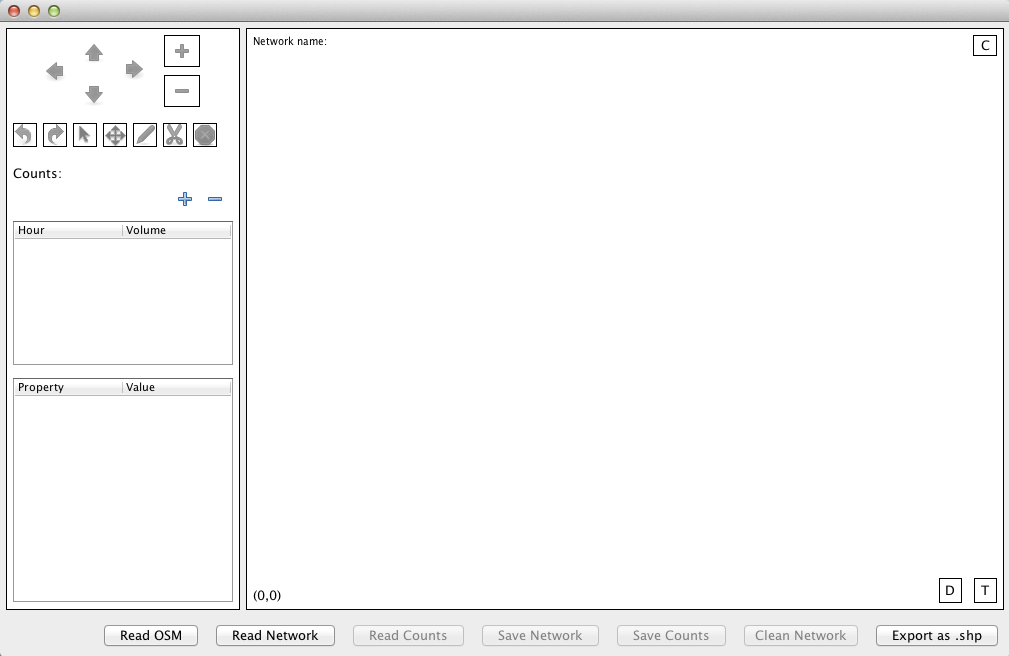
\includegraphics[width=\textwidth]{figures/networkEditor/emptyNetworkEditor.png}
\end{figure}

\subsubsection{Loading network data}

To load an existing MATSim network, click on the button "Read  Network" at the bottom of the window and select the network you want to  load.

Alternatively, you can import data from OpenStreetMap (OSM) and  automatically convert it into a network. For this, first download the  osm data for the region you're interested in. The \href{http://www.matsim.org/docs/tutorials/8lessons/input/creating/network}{tutorial}  contains information on how you can download the required data from  OSM. Once you have a *.osm file containing the data for your region,  click on the button "Read OSM" and select the file. When loading the  data, the following window will open:


\begin{figure}[htp]
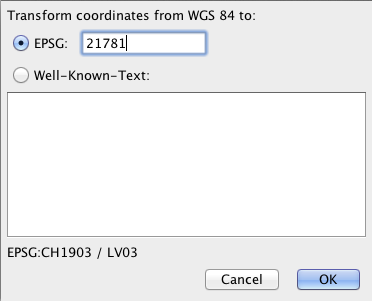
\includegraphics[width=0.6\textwidth]{figures/networkEditor/crsNetworkEditor.png}
\end{figure}

The original data from OSM contains coordinates in the WGS 84  coordinate reference system. WGS 84 is impractical to work with in  MATSim, so we need to convert the coordinates into another coordinate  reference system (CRS). In the example above, we convert it to the Swiss  national coordinate reference system. To find the corresponding EPSG  codes, or the Well-Known-Text description of your CRS, have a look at \href{http://spatialreference.org/}{http://spatialreference.org/} and search for your CRS.

Click OK to close the dialog once you have the correct CRS set. The  OSM data will now be converted and the network displayed afterwards in  the editor. Especially for larger osm files, have some patience for the  conversion process. It may take some while to convert the data and  finally show the network.

\subsubsection{Editing network}

Once a network is loaded, most of the tools in the upper left corner of the window become active:

\begin{figure}[htp]
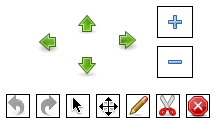
\includegraphics[width=.5\textwidth]{figures/networkEditor/toolsNetworkEditor.png}
\end{figure}

The 4 green arrows are to move the network around in the editor view.  The blue + and – are for zooming in and out. In the row below, the  buttons have the following functionality:
\begin{itemize}
	\item undo / redo: revert and redo changes you did to the network
	\item Selection: select a link or a node by clicking on them in the editor  view. click and drag to select multiple elements. If you have a single  link selected, you can change some of the link's attributes in the panel  on the lower left of the window.
	\item move view: click and drag the network to move the network in the editor view
	\item add link: click in a place to start a new link, click a second time  to end the link at that place. If the clicks are close to a node, the  link will start/end at that node, otherwise a new node will be created.
	\item divide a link: select a link first, then use the scissors to cut the  link into two. A new node will be added at the location of the click,  and the original link will be splitted into two parts.
	\item delete a link: select a link first, then click this button to delete  the selected link. If you clicked on the button by accident, use the  undo-button.
\end{itemize}

\subsubsection{Saving a network}

To save a network in MATSim's format, click on the button "Save  Network". Alternatively, you can export the network as a Shape file that  can be used by allmost all GIS applications for visualization purposes  (but not necessarily for network operations that some GIS applications  offer). Just click on "Export as Shp" to export the network as a Shape  file.

\subsubsection{Working with counts data}

Once you have a network loaded, you can optionally also load some  existing counts for this network. If you just converted your network  from OSM data, you likely won't have any such file. In that case, you  can directly start to add counts where you want. Select a link by  clicking on it. If the link already has counts associated, they will be  displayed in the panel on the left side of the window. Click the + there  to add count values, even if no counts exist yet for this link.

After you're done with the counts editing, save the counts to a file by clicking on "Save Counts".

